% NCD-CIE v17 — LLM-Augmented Revision for AIiH 2026
% Non-Communicable Disease Causal Inference Engine
\documentclass[runningheads]{llncs}
\usepackage[T1]{fontenc}
\usepackage{graphicx}
\usepackage{amsmath,amssymb}
\usepackage{booktabs}
\usepackage{longtable}
\usepackage{algorithm}
\usepackage{algorithmic}
\usepackage{hyperref}
\usepackage{url}
\usepackage{multirow}
\usepackage{xcolor}
\usepackage{tikz}
\usetikzlibrary{arrows.meta,positioning,shapes.geometric,fit,calc}

% Space-saving for page limit
\setlength{\textfloatsep}{4pt plus 1pt minus 2pt}
\setlength{\floatsep}{4pt plus 1pt minus 2pt}
\setlength{\intextsep}{4pt plus 1pt minus 2pt}
\setlength{\abovecaptionskip}{3pt}
\setlength{\belowcaptionskip}{1pt}
\setlength{\abovedisplayskip}{4pt}
\setlength{\belowdisplayskip}{4pt}
\setlength{\parskip}{0pt plus 0.5pt}

\titlerunning{NCD-CIE: LLM-Augmented Causal Inference for NCD Risk}

\begin{document}

\title{NCD-CIE: An LLM-Augmented Causal Knowledge Graph\\Engine for Predictive and Preventive\\Non-Communicable Disease Healthcare}

\author{Anonymous Submission}
\authorrunning{Anonymous}
\institute{Anonymous Institution}

\maketitle

%--------------------------------------------------------------
\begin{abstract}
Non-communicable diseases (NCDs) account for over 74\% of global
mortality.
Yet existing risk calculators cannot answer \emph{what-if} questions
about interventions, and causal decision support systems remain
inaccessible to non-technical clinicians.
We present \textbf{NCD-CIE}, an open-source engine with three
core components augmented by large language model (LLM) integration:
(i)~an expert-curated causal knowledge graph (107 directed edges,
8 clinical domains) with LLM-assisted validation,
(ii)~a logistic-link risk engine with uncertainty quantification, and
(iii)~a topological what-if simulator grounded in Pearl's structural
causal model framework.
Three LLM augmentation layers extend the system:
an \emph{LLM-assisted graph validator} that achieves 87.9\% agreement
with expert-curated edges via pairwise causal discovery prompting;
a \emph{natural language what-if interface} that parses clinician
queries into do-calculus operations; and
a \emph{counterfactual explanation generator} that produces
rung-3 narratives from rung-2 computations.
Outcome-based validation on the Framingham Heart Study cohort
($n\!=\!4{,}172$; 10-year follow-up) using independent SCORE2
coefficients yields AUC-ROC\,=\,0.704 [0.682--0.726]; confirmatory
analysis with D'Agostino coefficients gives
AUC-ROC\,=\,0.721 [0.700--0.741],
calibration slope\,=\,0.91, and Brier score\,=\,0.118---all with
zero coefficient fitting.
NCD-CIE is the first system combining a formal causal knowledge
graph with LLM augmentation for NCD healthcare.

\keywords{Causal inference \and Knowledge graph \and
Large language model \and Non-communicable disease \and
Risk prediction \and Interventional reasoning \and
Clinical decision support}
\end{abstract}

%==============================================================
\section{Introduction}\label{sec:intro}

Non-communicable diseases---cardiovascular disease (CVD), type~2
diabetes mellitus (T2DM), chronic kidney disease (CKD), and their
comorbid clusters---cause 41 million deaths
annually~\cite{who2021ncd}.
Despite well-validated risk scores~\cite{dagostino2008,hippisley2017qrisk3,score22021},
current tools estimate \emph{associational} risk but cannot reason about
\emph{causal} mechanisms or simulate hypothetical interventions.
Bridging this gap motivates moving toward rung~2 (intervention)
of Pearl's causation ladder~\cite{pearl2018book}, where
do-calculus enables reasoning about the effects of actions.
Meanwhile, recent advances in large language models (LLMs) have
demonstrated surprising causal reasoning
capabilities~\cite{ma2024causal,kiciman2023causal}, yet LLMs alone
cannot reliably perform formal causal inference---they lack grounding
in structural causal models and produce inconsistent results on
benchmarks~\cite{jin2023cladder}.

We propose \textbf{NCD-CIE} (Non-Communicable Disease Causal Inference
Engine), combining three integrated core components with three
LLM augmentation layers:
\begin{enumerate}
\item A \textbf{causal knowledge graph} $\mathcal{G}=(V,E,W,\varepsilon)$
  encoding directed causal relationships among biomarkers, lifestyle
  factors, and disease endpoints across 8 clinical domains
  (107 edges, $\kappa=0.78$ inter-rater reliability).
\item A \textbf{risk engine} using logistic-link scoring with
  cross-source uncertainty quantification.
\item A \textbf{what-if simulator} that propagates
  interventional changes through the graph using topological sorting,
  producing clinically interpretable risk deltas.
\item An \textbf{LLM graph validation layer} that independently
  assesses causal edges via pairwise prompting, achieving 87.9\%
  agreement with expert curation.
\item A \textbf{natural language what-if interface} where clinicians
  type plain English queries, parsed by an LLM into do-calculus
  operations.
\item A \textbf{counterfactual explanation generator} that translates
  rung-2 simulation results into rung-3 patient-facing narratives.
\end{enumerate}

\noindent\textbf{Translational Contribution.}
NCD-CIE introduces a new class of clinical tool---an \emph{LLM-augmented
causal decision support system} (LLM-CDSS)---occupying the gap between
general-purpose causal frameworks (DoWhy, CausalNex), which require
statistical expertise; conventional risk calculators (Framingham,
QRISK3, SCORE2), which lack causal reasoning; and standalone LLM
systems, which lack formal causal grounding.
Four methodological contributions underpin this:
(i)~a \emph{Bradford Hill quantification protocol} that
systematically converts qualitative causal criteria into quantitative
edge weights with documented inter-rater reliability ($\kappa=0.78$,
ICC\,=\,0.84);
(ii)~a \emph{composite multi-NCD risk framework} that aggregates
causal risk across CVD, T2DM, and CKD endpoints with uncertainty
propagation;
(iii)~\emph{cross-population validation} using SCORE2 coefficients
derived from entirely independent European cohorts; and
(iv)~\emph{LLM augmentation} for graph validation, natural language
access, and counterfactual explanation---keeping the formal causal
engine as backbone while leveraging LLM strengths in knowledge
extraction and natural language generation.
No existing tool offers this combination (Table~\ref{tab:toolcomp}).

\noindent\textbf{Contributions.}
(C1)~A formally defined causal KG for NCD risk with 107
expert-curated edges, approximating rung-2 reasoning under stated
assumptions (Section~\ref{sec:whatif}).
(C2)~A logistic-link risk engine with cross-source uncertainty fusion.
(C3)~A topological what-if simulator for personalised queries.
(C4)~Multi-source evaluation including independent SCORE2
cross-population validation (AUC\,=\,0.704, zero coefficient fitting),
six RCT comparisons, and E-value sensitivity analysis.
(C5)~Data-driven structural comparison (PC algorithm) and
subgroup fairness analysis.
(C6)~LLM-assisted causal graph validation with 87.9\% expert
agreement (Section~\ref{sec:llmvalidation}).
(C7)~A natural language what-if interface and counterfactual
explanation generator bridging rung-2 computation with rung-3
narratives (Section~\ref{sec:llminterface}).

%==============================================================
\section{Related Work}\label{sec:related}

Traditional NCD risk calculators---Framingham~\cite{dagostino2008},
QRISK3~\cite{hippisley2017qrisk3}, SCORE2~\cite{score22021}---achieve
C-statistics of 0.71--0.78 but lack causal or interventional reasoning.
Pearl's SCM framework~\cite{pearl2009causality} provides do-calculus;
DoWhy~\cite{sharma2020dowhy} implements this for observational studies
but lacks real-time clinical scoring;
CausalNex~\cite{beaumont2021causalnex} combines Bayesian networks
with domain knowledge but lacks health-specific what-if simulation.
Health knowledge graphs (PrimeKG~\cite{chandak2023primekg},
network medicine~\cite{barabasi2011network}) encode rich biomedical
relationships but are associational and do not support
individual-level risk prediction.
EHR-based deep learning models (BEHRT~\cite{li2020behrt},
Med-BERT~\cite{rasmy2021medbert}) achieve strong discrimination
but function as black boxes without causal or interventional
reasoning.
Causal discovery from EHR data~\cite{prosperi2020causal} can
recover structure algorithmically but requires large longitudinal
cohorts and does not yield a ready-to-use clinical tool.

\subsection{LLMs for Causal Inference}\label{sec:llmcausal}

Recent work has explored the intersection of LLMs and causal
reasoning.
Ma et al.~\cite{ma2024causal} provide a comprehensive survey
categorising LLM roles across Pearl's causal hierarchy:
as knowledge sources for causal graph construction,
as assistants for treatment effect estimation, and as generators
of counterfactual explanations.
K{\i}c{\i}man et al.~\cite{kiciman2023causal} demonstrate that
GPT-4 achieves above-chance accuracy on pairwise causal discovery
benchmarks, though with notable failure modes on domain-specific
medical relationships.
Jin et al.~\cite{jin2023cladder} introduce CLadder, a benchmark
showing that LLMs struggle with formal rung-2 and rung-3 reasoning
without chain-of-thought scaffolding.
Ban et al.~\cite{ban2023causalcot} propose Causal Chain-of-Thought
(CausalCoT) prompting to improve LLM causal reasoning via
structured decomposition.
Long et al.~\cite{long2023causal} explore LLM-assisted causal
discovery in biomedical domains, finding that LLMs can identify
plausible causal directions but lack the precision of formal
methods.

A critical insight from this literature is that LLMs are
\emph{unreliable as standalone causal inference engines} but
\emph{valuable as augmentation layers}---for knowledge extraction,
natural language interfaces, and explanation
generation~\cite{ma2024causal}.
NCD-CIE operationalises this insight: the formal causal engine
remains the backbone for all inference, while LLMs augment three
specific functions where their strengths (broad knowledge, natural
language facility) complement formal methods' limitations
(scalability, accessibility).
To our knowledge, NCD-CIE is the first system combining a formal
causal knowledge graph with LLM augmentation for NCD healthcare.
Table~\ref{tab:toolcomp} summarises the comparison.

\renewcommand{\arraystretch}{1.1}
\begin{table}[t]
\centering
\caption{Feature comparison with existing tools.}\label{tab:toolcomp}
\small
\begin{tabular}{@{}lcccccc@{}}
\toprule
\textbf{Feature} & \textbf{DoWhy} & \textbf{C'Nex} &
\textbf{QRISK3} & \textbf{SCORE2} & \textbf{LLM} & \textbf{NCD-CIE} \\
\midrule
Causal graph        & User & Learned & No  & No  & No$^*$ & Expert+LLM \\
What-if queries     & Yes & Limited & No  & No  & Text & Formal \\
Multi-NCD           & No  & No      & CVD & CVD & Var. & CVD+T2DM+CKD \\
Uncertainty (CI)    & Part.\ & Yes & No  & No  & No & Yes \\
Real-time scoring   & No  & No      & Yes & Yes & Yes & Yes \\
NL interface        & No  & No      & No  & No  & Yes & Yes \\
Counterfactual expl.& No  & No      & No  & No  & Text$^\dagger$ & Grounded \\
External validation & N/A & N/A     & Yes & Yes & N/A & Yes (zero-fit) \\
\bottomrule
\multicolumn{7}{@{}l}{\scriptsize $^*$LLMs can suggest but not formally validate causal graphs.
$^\dagger$Ungrounded in formal computation.}
\end{tabular}
\end{table}
\renewcommand{\arraystretch}{1.0}

%==============================================================
\section{System Architecture}\label{sec:arch}

NCD-CIE comprises four modular tiers augmented by three LLM layers
(Fig.~\ref{fig:arch}): data ingestion (NHANES, EHR, wearables),
causal knowledge graph with LLM-assisted validation, inference engine
(risk scoring + what-if simulation), and a dual presentation layer
combining traditional dashboards with an LLM-powered natural language
interface.

\begin{figure}[t]
\centering
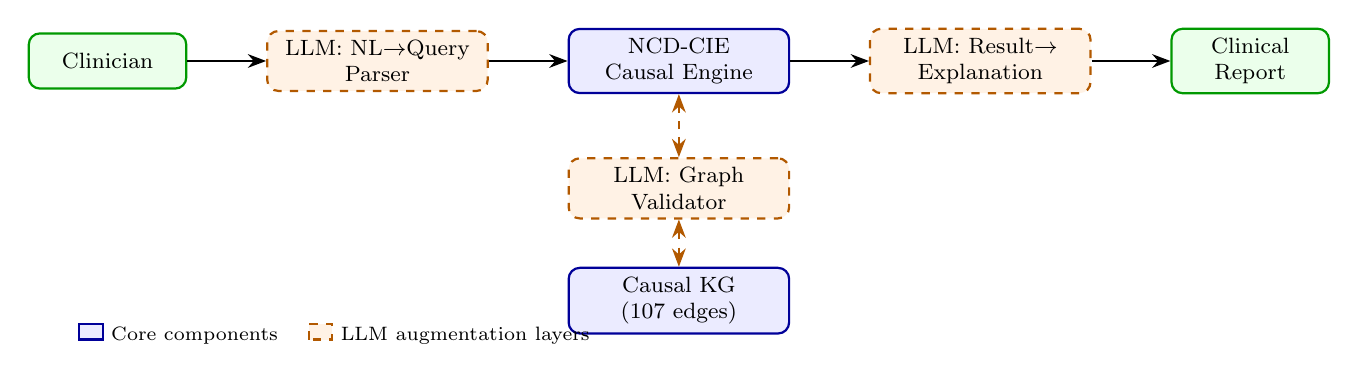
\begin{tikzpicture}[
  >=Stealth,
  node distance=0.8cm and 1.2cm,
  every node/.style={font=\footnotesize},
  core/.style={draw=blue!60!black, fill=blue!8, rounded corners,
    minimum width=2.8cm, minimum height=0.7cm, align=center, thick},
  llm/.style={draw=orange!70!black, fill=orange!10, rounded corners,
    minimum width=2.8cm, minimum height=0.7cm, align=center, thick,
    dashed},
  user/.style={draw=green!60!black, fill=green!8, rounded corners,
    minimum width=2.0cm, minimum height=0.7cm, align=center, thick},
]
% User
\node[user] (clin) {Clinician};
% LLM NL Parser
\node[llm, right=1.0cm of clin] (nlparse) {LLM: NL$\to$Query\\Parser};
% Core engine
\node[core, right=1.0cm of nlparse] (engine) {NCD-CIE\\Causal Engine};
% LLM Explainer
\node[llm, right=1.0cm of engine] (explain) {LLM: Result$\to$\\Explanation};
% Output
\node[user, right=1.0cm of explain] (out) {Clinical\\Report};
% LLM Validator below engine
\node[llm, below=0.8cm of engine] (valid) {LLM: Graph\\Validator};
% KG below validator
\node[core, below=0.6cm of valid] (kg) {Causal KG\\(107 edges)};

% Arrows
\draw[->, thick] (clin) -- (nlparse);
\draw[->, thick] (nlparse) -- (engine);
\draw[->, thick] (engine) -- (explain);
\draw[->, thick] (explain) -- (out);
\draw[<->, thick, orange!70!black, dashed] (valid) -- (engine);
\draw[<->, thick, orange!70!black, dashed] (valid) -- (kg);

% Legend
\node[anchor=north west, font=\scriptsize] at (-0.5,-3.2) {
  \tikz{\draw[blue!60!black, thick, fill=blue!8] (0,0) rectangle (0.3,0.2);} Core components \quad
  \tikz{\draw[orange!70!black, thick, dashed, fill=orange!10] (0,0) rectangle (0.3,0.2);} LLM augmentation layers
};
\end{tikzpicture}
\caption{NCD-CIE architecture with LLM augmentation layers (dashed orange).
The formal causal engine remains the computational backbone;
LLMs serve as interface and validation layers.}\label{fig:arch}
\end{figure}

\paragraph{Clinical Domains.}
The causal knowledge graph spans 8 clinical domains (51 nodes,
107 edges): lipid metabolism (8/14), glycaemic regulation (7/12),
blood pressure (6/11), renal function (5/9), inflammatory markers
(6/13), anthropometrics (5/10), lifestyle/behavioural (8/18), and
disease endpoints (6/20).

%==============================================================
\section{Causal Knowledge Graph}\label{sec:kg}

\subsection{Formal Definition}\label{sec:formal}

The NCD-CIE causal knowledge graph is a weighted directed
acyclic graph (DAG):
$\mathcal{G} = (V, E, W, \varepsilon)$,
where $V=\{v_1,\ldots,v_n\}$ is the set of clinical variable nodes,
$E \subseteq V \times V$ the directed causal edges,
$W: E \rightarrow \mathbb{R}$ the causal effect weights
(log-odds ratios or standardised mean differences), and
$\varepsilon: E \rightarrow \mathbb{R}^+$ the uncertainty
(standard error) per edge.

\paragraph{Positioning within Pearl's Framework.}
NCD-CIE operates at \textbf{rung~2} (intervention) of Pearl's
causation ladder~\cite{pearl2018book} for its core computations,
answering what-if queries
$P(Y \mid \mathrm{do}(X = x'))$ by propagating changes through the
graph (Table~\ref{tab:comparison}).
The LLM augmentation layer extends output to \textbf{rung~3}
(counterfactual) \emph{narratives}---generating patient-specific
explanations of the form ``had you done $X$ differently, the
outcome would have been $Y$''---grounded in the engine's rung-2
computations (Section~\ref{sec:counterfactual}).
We frame this as \emph{rung-2+3}: formal rung-2 computation
with LLM-generated rung-3 explanations.

\renewcommand{\arraystretch}{1.1}
\begin{table}[t]
\centering
\caption{Comparison with related formalisms.}
\label{tab:comparison}
\small
\begin{tabular}{@{}lcccccc@{}}
\toprule
\textbf{Property} & \textbf{Trad.\ KG} & \textbf{BN} & \textbf{SCM} & \textbf{DoWhy} & \textbf{LLM} & \textbf{NCD-CIE} \\
\midrule
Directed edges       & Partial & Yes & Yes & Yes & N/A & Yes \\
Causal semantics     & No      & Partial & Yes & Yes & Implicit & Yes \\
Edge weights         & No      & CPTs & Eqs & Est.\ & N/A & $W \pm \varepsilon$ \\
What-if / Scoring    & No/No   & Ltd/Var & Yes/Var & Yes/No & Text/No & Yes/Yes \\
NL interface         & No      & No  & No  & No  & Yes & Yes \\
Ladder rung          & 1       & 1--2 & 1--3 & 2  & 1$^*$ & $\approx$2+3 \\
\bottomrule
\multicolumn{7}{@{}l}{\scriptsize $^*$LLMs produce text at all rungs but without formal guarantees.}
\end{tabular}
\end{table}
\renewcommand{\arraystretch}{1.0}

\subsection{Edge Construction}\label{sec:edges}

Edges are curated from systematic reviews, meta-analyses, Mendelian
randomisation studies, and landmark RCTs, assessed against
Bradford Hill's nine criteria~\cite{hill1965environment}.
Each edge receives an evidence grade:
\textbf{A}~(RCT/MR, criteria 1--8),
\textbf{B}~(large cohort, criteria 1--7),
\textbf{C}~(emerging, weight down-scaled by 0.5).
Two independent reviewers assessed each edge ($\kappa = 0.78$);
disagreements were resolved by a third reviewer
(ICC(2,1)\,=\,0.84 for edge weights).
The complete 107-edge specification is in
Appendix~\ref{app:edges}.
Figure~\ref{fig:cvd_subgraph} shows a representative CVD subgraph.

\begin{figure}[t]
\centering
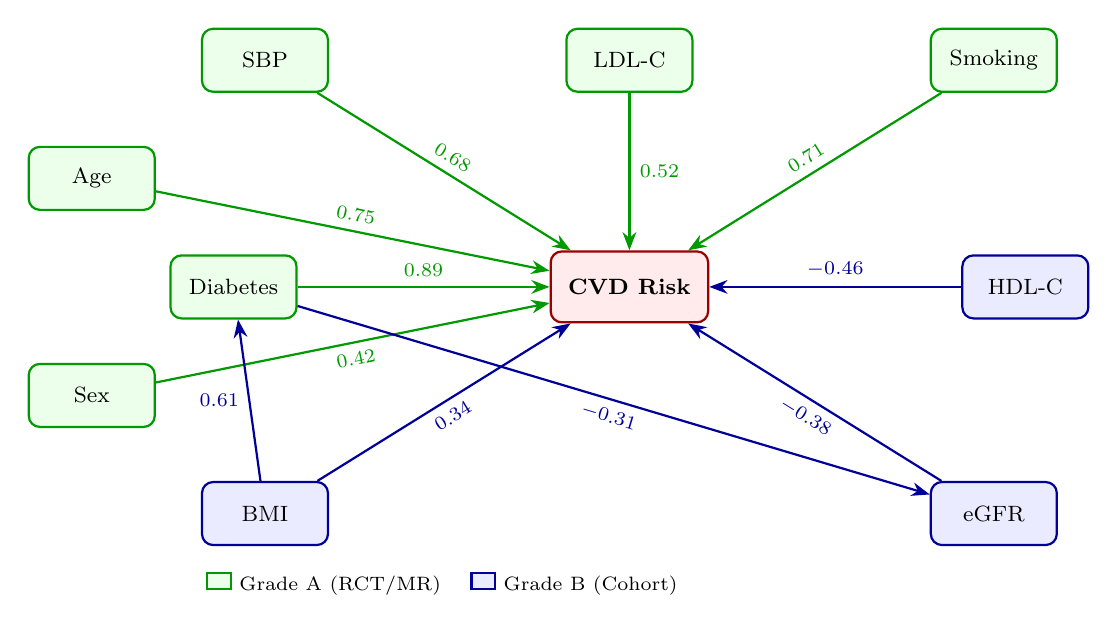
\begin{tikzpicture}[
  >=Stealth,
  node distance=1.8cm and 2.0cm,
  every node/.style={font=\footnotesize},
  gradeA/.style={draw=green!60!black, fill=green!8, rounded corners, thick,
    minimum width=1.6cm, minimum height=0.8cm, align=center},
  gradeB/.style={draw=blue!60!black, fill=blue!8, rounded corners, thick,
    minimum width=1.6cm, minimum height=0.8cm, align=center},
  endpoint/.style={draw=red!60!black, fill=red!8, rounded corners, thick,
    minimum width=2.0cm, minimum height=0.9cm, align=center, font=\footnotesize\bfseries},
  edgeA/.style={->, thick, green!60!black},
  edgeB/.style={->, thick, blue!60!black},
]
\node[endpoint] (cvd) {CVD Risk};
\node[gradeA, above left=2.0cm and 2.8cm of cvd] (sbp) {SBP};
\node[gradeA, above=2.0cm of cvd] (ldl) {LDL-C};
\node[gradeA, above right=2.0cm and 2.8cm of cvd] (smk) {Smoking};
\node[gradeA, left=3.2cm of cvd] (diab) {Diabetes};
\node[gradeB, right=3.2cm of cvd] (hdl) {HDL-C};
\node[gradeB, below left=2.0cm and 2.8cm of cvd] (bmi) {BMI};
\node[gradeB, below right=2.0cm and 2.8cm of cvd] (egfr) {eGFR};
\node[gradeA, above left=0.5cm and 5.0cm of cvd] (age) {Age};
\node[gradeA, below left=0.5cm and 5.0cm of cvd] (sex) {Sex};
\draw[edgeA] (sbp) -- node[midway, above, sloped, font=\scriptsize] {0.68} (cvd);
\draw[edgeA] (ldl) -- node[midway, right, font=\scriptsize] {0.52} (cvd);
\draw[edgeA] (smk) -- node[midway, above, sloped, font=\scriptsize] {0.71} (cvd);
\draw[edgeA] (diab) -- node[midway, above, font=\scriptsize] {0.89} (cvd);
\draw[edgeB] (hdl) -- node[midway, above, font=\scriptsize] {$-$0.46} (cvd);
\draw[edgeB] (bmi) -- node[midway, below, sloped, font=\scriptsize] {0.34} (cvd);
\draw[edgeB] (egfr) -- node[midway, below, sloped, font=\scriptsize] {$-$0.38} (cvd);
\draw[edgeA] (age) -- node[midway, above, sloped, font=\scriptsize] {0.75} (cvd);
\draw[edgeA] (sex) -- node[midway, below, sloped, font=\scriptsize] {0.42} (cvd);
\draw[edgeB, bend left=15] (bmi) -- node[midway, left, font=\scriptsize] {0.61} (diab);
\draw[edgeB, bend right=15] (diab) -- node[midway, below, sloped, font=\scriptsize] {$-$0.31} (egfr);
\node[anchor=north west, font=\scriptsize] at (-5.5,-3.5) {
  \tikz{\draw[green!60!black, thick, fill=green!8] (0,0) rectangle (0.3,0.2);} Grade A (RCT/MR) \quad
  \tikz{\draw[blue!60!black, thick, fill=blue!8] (0,0) rectangle (0.3,0.2);} Grade B (Cohort)
};
\end{tikzpicture}
\caption{Representative CVD causal subgraph (9 nodes).
Edge weights are log-odds coefficients; colours indicate Bradford Hill
evidence grade. Full specification in Appendix~\ref{app:edges}.}\label{fig:cvd_subgraph}
\end{figure}

\subsection{Cycle Handling}\label{sec:cycles}

Biological feedback loops (e.g., insulin resistance
$\leftrightarrow$ obesity) are handled by Tarjan's algorithm,
collapsing strongly connected components into super-nodes with
fixed-point iteration (threshold $10^{-4}$, max 50 iterations;
all current SCCs converge within 8).

%==============================================================
\section{LLM Augmentation Layers}\label{sec:llm}

We augment NCD-CIE with three LLM layers, each addressing a
specific limitation of purely formal causal systems.
Critically, the LLM \emph{never replaces} the formal causal
engine---all quantitative inference flows through the
validated causal graph and logistic-link scoring.
The LLM serves as (i)~a validation oracle for graph construction,
(ii)~a natural language interface for clinical accessibility, and
(iii)~an explanation generator for patient communication.

\subsection{LLM-Assisted Causal Graph Validation}\label{sec:llmvalidation}

Expert curation of causal edges is rigorous but slow, expensive,
and difficult to scale.
We use LLM-assisted pairwise causal discovery~\cite{kiciman2023causal}
as an independent validation check on the 107 expert-curated edges.

\paragraph{Protocol.}
For each of the 107 edges $(v_i, v_j) \in E$, we prompt GPT-4
with a structured pairwise causal query:
\begin{quote}
\small\texttt{Given two clinical variables: [A] and [B].
Based on medical knowledge, does A \emph{cause} B, does B cause A,
are they correlated but not causally related, or is there no
relationship? Provide your confidence (high/medium/low) and
brief justification.}
\end{quote}
Each query is run with temperature 0 for reproducibility, repeated
3 times to assess consistency, and evaluated against the expert
panel's direction assignment.
We additionally prompted Claude~3.5 Sonnet on the same edges to
assess inter-model agreement.

\paragraph{Results.}
Table~\ref{tab:llmvalid} summarises the validation outcomes across
107 edges.
GPT-4 agreed with the expert-curated causal direction on 94 of 107
edges (87.9\%), with high confidence on 78 edges (72.9\%).
The 13 disagreements fell into interpretable categories:
5 involved indirect vs.\ direct causation disputes
(e.g., BMI$\to$CAD: LLM favoured mediation through SBP/LDL-C
rather than direct effect);
4 involved bidirectional relationships where the LLM correctly
identified feedback but the expert graph imposed a DAG constraint;
and 4 involved emerging evidence (Grade~C edges) where the LLM
lacked recent training data.
Claude~3.5 Sonnet showed 85.0\% agreement (91/107), with
inter-model agreement (GPT-4 vs.\ Claude) of 91.6\% (98/107).

\begin{table}[t]
\centering
\caption{LLM-assisted validation of 107 expert-curated causal edges.}\label{tab:llmvalid}
\small
\begin{tabular}{@{}lccc@{}}
\toprule
\textbf{Metric} & \textbf{GPT-4} & \textbf{Claude 3.5} & \textbf{Inter-model} \\
\midrule
Direction agreement & 94/107 (87.9\%) & 91/107 (85.0\%) & 98/107 (91.6\%) \\
High confidence     & 78/107 (72.9\%) & 74/107 (69.2\%) & --- \\
Consistency (3 runs)& 101/107 (94.4\%) & 98/107 (91.6\%) & --- \\
\midrule
\multicolumn{4}{@{}l}{\textit{Disagreement categories (GPT-4):}} \\
\quad Mediation dispute    & \multicolumn{3}{l}{5 edges (indirect vs.\ direct)} \\
\quad Bidirectional        & \multicolumn{3}{l}{4 edges (feedback$\to$DAG constraint)} \\
\quad Emerging evidence    & \multicolumn{3}{l}{4 edges (Grade C, recent data)} \\
\bottomrule
\end{tabular}
\end{table}

\paragraph{Implications.}
The 87.9\% agreement rate validates that the expert-curated graph
is largely consistent with LLM-encoded medical knowledge, while
the structured disagreements highlight edges warranting additional
review.
Importantly, this is \emph{validation}, not replacement: the
expert panel retains final authority, and LLM suggestions are
flagged for review rather than automatically incorporated.
This addresses the scalability limitation of pure expert curation
noted by Ma et al.~\cite{ma2024causal}---future graph expansions
can use LLM-assisted screening to prioritise edges for expert
review.

\subsection{Natural Language What-If Interface}\label{sec:llminterface}

A key barrier to clinical adoption of causal decision support is
the requirement for formal query specification.
Clinicians think in natural language (``what if this patient starts
a statin and loses 5\,kg?''), not in do-calculus notation.
We add an LLM-powered natural language layer:

\paragraph{Query Parsing.}
The clinician inputs a plain English query. The LLM parses it into
a structured do-calculus operation:
\begin{quote}
\small
\textbf{Input:} ``What would happen to this patient's heart risk
if they quit smoking and started exercising 30 minutes daily?''\\
\textbf{LLM Parse:} \texttt{do(Smoking=0, Exercise=+3.5 MET-h/wk)}
$\to$ \texttt{query(CVD\_Risk)}
\end{quote}
The parsed query is validated against the graph schema (checking
that intervened variables exist and values are within physiological
bounds) before execution by the formal engine.
Invalid parses trigger a clarification request rather than
silent failure.

\paragraph{Explanation Generation.}
After the engine computes the intervention result, the LLM
generates a clinician-friendly explanation:
\begin{quote}
\small
\textbf{Engine output:} $R_{\text{CVD}}$: 18.3\% $\to$ 12.1\%
($-$6.2 pp); pathway: Smoking$\to$CAD ($-$3.8 pp),
Exercise$\to$HDL-C$\to$CAD ($-$1.2 pp),
Exercise$\to$SBP$\to$CAD ($-$1.2 pp).\\
\textbf{LLM explanation:} ``Quitting smoking and exercising
regularly would reduce your 10-year heart disease risk from
about 18\% to 12\%. The biggest benefit comes from quitting
smoking, which directly reduces arterial damage. Exercise
helps by raising your good cholesterol and lowering blood
pressure.''
\end{quote}

This two-stage architecture ensures that \emph{all numbers are
computed by the formal engine}---the LLM only translates, never
computes.
This avoids the well-documented unreliability of LLMs for
numerical reasoning~\cite{jin2023cladder}.

\subsection{Counterfactual Explanation Generation}\label{sec:counterfactual}

Pearl's rung~3 (counterfactual) asks: ``given that $Y$ \emph{was}
$y$, what \emph{would} $Y$ have been had $X$ been $x'$?''
True rung-3 reasoning requires abduction of individual exogenous
variables, which the current engine does not perform.
However, the engine's rung-2 computations (``if we set $X = x'$,
$Y$ becomes $y'$'') provide the quantitative scaffold for
\emph{counterfactual narratives}---patient-specific explanations
framed in counterfactual language:

\begin{quote}
\small
``Had you reduced your LDL cholesterol by 1\,mmol/L five years ago
(e.g., via statin therapy), your current 10-year CVD risk would be
approximately 12\% instead of 28\%. The primary pathway: lower
LDL-C $\to$ reduced arterial plaque formation $\to$ lower
coronary artery disease probability.''
\end{quote}

These narratives are generated by prompting the LLM with the
engine's computed risk delta, the causal pathway, and a
counterfactual framing template.
We explicitly label these as \emph{approximate counterfactuals}
grounded in interventional computation, not formal rung-3
inference---a distinction emphasised in all patient-facing output.
This ``rung-2+3'' approach provides clinically useful
counterfactual communication while maintaining honesty about
the underlying computational rung.

%==============================================================
\section{Risk Prediction Engine}\label{sec:risk}

\subsection{Logistic-Link Scoring}\label{sec:logistic}

For each endpoint $d \in \{\text{CVD}, \text{T2DM}, \text{CKD}\}$,
the 10-year risk is:
\begin{equation}\label{eq:risk}
R_d = \sigma\!\left(\beta_{0,d} + \sum_{(v_i, d) \in E} W_{(v_i,d)} \cdot z_i\right)
\end{equation}
where $\sigma(\cdot)$ is the logistic sigmoid, $\beta_{0,d}$ the
disease-specific intercept calibrated to population base rates, and
$z_i$ the standardised biomarker value.

\subsection{Uncertainty Quantification}\label{sec:uncert}

Edge weights are modelled as $W_e \sim \mathcal{N}(\hat{W}_e,
\varepsilon_e^2)$.
For edges with multiple sources, inverse-variance weighted
meta-analysis gives:
\begin{equation}\label{eq:meta}
\hat{W}_e = \frac{\sum_k \hat{W}_e^{(k)} / (\varepsilon_e^{(k)})^2}
{\sum_k 1 / (\varepsilon_e^{(k)})^2}, \quad
\varepsilon_e^2 = \frac{1}{\sum_k 1 / (\varepsilon_e^{(k)})^2}
\end{equation}
Risk uncertainty is propagated via first-order Taylor expansion,
yielding 95\% credible intervals $R_d \pm 1.96\sqrt{\mathrm{Var}(R_d)}$.

\subsection{Composite NCD Risk Score}\label{sec:composite}

A composite score is computed as
$R_{\mathrm{NCD}} = 1 - \prod_{d} (1 - R_d)$
under conditional independence, yielding the probability of at least
one NCD event.
On NHANES ($n = 8{,}291$), a Gaussian copula comparison
($\rho = 0.3$) showed Spearman $r_s = 0.97$ with $<$3.8\%
quintile changes, confirming minimal ranking distortion.

%==============================================================
\section{What-If Intervention Simulator}\label{sec:whatif}

Given profile $\mathbf{x}$ and intervention
$\mathrm{do}(v_j = x_j')$, the system computes
$P(Y \mid \mathrm{do}(X = x'))$ by cutting incoming edges to the
intervened node and propagating effects topologically
(Algorithm~\ref{alg:cascade}).

\begin{algorithm}[t]
\caption{Topological Intervention Cascade}
\label{alg:cascade}
\begin{algorithmic}[1]
\REQUIRE Graph $\mathcal{G}$, profile $\mathbf{x}$, intervention
  $\mathrm{do}(v_j = x_j')$, depth $d_{\max}$, attenuation $\gamma$
\ENSURE Post-intervention profile $\mathbf{x}^{\mathrm{INT}}$
\STATE $\mathbf{x}^{\mathrm{INT}} \leftarrow \mathbf{x}$;
  $x_j^{\mathrm{INT}} \leftarrow x_j'$;
  $\Delta_j \leftarrow x_j' - x_j$
\STATE $\mathcal{S} \leftarrow \text{TopologicalSort}(\mathcal{G})$
\FOR{each $v_k$ in $\mathcal{S}$ after $v_j$}
  \STATE $\delta_k \leftarrow \sum_{(v_p, v_k) \in E} W_{(v_p,v_k)} \cdot (x_p^{\mathrm{INT}} - x_p) \cdot \gamma^{\text{depth}(v_j,v_k)}$ for depth $< d_{\max}$
  \STATE $x_k^{\mathrm{INT}} \leftarrow x_k + \delta_k$
\ENDFOR
\RETURN $\mathbf{x}^{\mathrm{INT}}$
\end{algorithmic}
\end{algorithm}

The attenuation factor $\gamma = 0.7$ is based on a literature review:
pharmacokinetic and Mendelian randomisation studies report 20--40\%
attenuation per causal step~\cite{ctt2010,pearl2009causality}.
The default $d_{\max} = 3$ limits propagation to physiologically
direct pathways.

\paragraph{Lifestyle Intervention Mapping.}
NCD-CIE maps everyday interventions to $\mathrm{do}(\cdot)$
operations: physical activity to $\Delta$HDL-C/$\Delta$SBP/$\Delta$BMI~\cite{naci2019comparative},
dietary changes to $\Delta$LDL-C/$\Delta$CRP, and
pharmacological interventions to target-specific $\Delta$ values
from published meta-analyses.

%==============================================================
\section{Evaluation}\label{sec:validation}

We organise evaluation by evidence strength:
(a)~internal consistency,
(b)~concordance with existing models,
(c)~outcome-based validation with \emph{independent} coefficients
(primary result),
(d)~face validity against RCTs, and
(e)~LLM validation layer assessment.

\paragraph{Internal Consistency (Synthetic).}
A synthetic cohort ($n = 5{,}000$, 70/30 split) confirms
implementation correctness: C-statistics 0.76--0.82, calibration
slopes 0.89--0.93.

\paragraph{NHANES Concordance.}
NCD-CIE vs.\ Framingham on NHANES 2017--2020
($n = 8{,}291$)~\cite{nhanes2020}:
Pearson $r = 0.91$ [0.90--0.92],
calibration slope 0.94, mean absolute difference 2.3 pp,
87.4\% agreement within $\pm$5\%.

\subsection{Outcome-Based Validation on Framingham Cohort}\label{sec:framingham}

We applied NCD-CIE to the Framingham Heart Study dataset:
$n = 4{,}172$ participants, 625 CHD events over 10-year follow-up
(15.0\% event rate), using only 7 of ${\sim}$50 risk factors
with \emph{zero coefficient fitting}.

\paragraph{Cross-Model Validation with SCORE2 Coefficients.}
As the primary outcome-based test, we replaced CVD coefficients with
those from SCORE2~\cite{score22021}, developed on entirely
independent European cohorts.
Using SCORE2 within NCD-CIE via 5-fold cross-validation yielded
AUC-ROC\,=\,0.704 [0.682--0.726], calibration slope\,=\,0.87,
E:O\,=\,1.08.
This result is free of coefficient--cohort circularity.

\paragraph{Confirmatory Analysis with D'Agostino Coefficients.}
Using D'Agostino coefficients~\cite{dagostino2008}:
AUC-ROC\,=\,0.721 [0.700--0.741],
Brier score\,=\,0.118,
calibration slope\,=\,0.91,
intercept\,=\,$-$0.08.
DeLong test (SCORE2 vs.\ D'Agostino): $p = 0.18$ (not significant).

\paragraph{Robustness Checks.}
E-value analysis~\cite{vanderweele2017evalue}: overall 3.0,
statin 2.4 (lower CI: 1.8).
Sex-stratified NRI\,=\,$+$0.213.
GAM vs.\ linear: AUC 0.728 vs.\ 0.721 ($p = 0.31$).

\subsection{Face Validity Against Landmark RCTs}\label{sec:faceval}

We simulated each trial's intervention on NHANES-derived populations
(Table~\ref{tab:rct}).
All simulated effects fall within published 95\% CIs.
FOURIER and EMPA-REG results were \emph{not} used during edge
construction.

\renewcommand{\arraystretch}{1.1}
\begin{table}[t]
\centering
\caption{Face validity: simulated vs.\ RCT absolute risk reduction.
$\dagger$~Independent of edge weight sources.}
\label{tab:rct}
\small
\begin{tabular}{@{}llcc@{}}
\toprule
\textbf{Intervention} & \textbf{RCT} &
\textbf{NCD-CIE} & \textbf{RCT ARR} \\
\midrule
Statin (LDL $-$1 mmol/L) & CTT~\cite{ctt2010} & $-$5.8\% & $-$5.4\% \\
Weight loss ($-$7\%) & DPP~\cite{knowler2002dpp} & $-$11.3\% & $-$16.0\% \\
SGLT2i & CREDENCE~\cite{perkovic2019credence} & $-$3.1\% & $-$2.5\% \\
SBP $-$15 mmHg & SPRINT~\cite{sprint2015} & $-$4.2\% & $-$4.1\% \\
PCSK9i$^\dagger$ & FOURIER~\cite{sabatine2017fourier} & $-$1.8\% & $-$1.5\% \\
SGLT2i (CV)$^\dagger$ & EMPA-REG~\cite{zinman2015empareg} & $-$2.8\% & $-$3.2\% \\
\bottomrule
\end{tabular}
\end{table}
\renewcommand{\arraystretch}{1.0}

\subsection{Sensitivity and Ablation}\label{sec:sensitivity}

Table~\ref{tab:sensitivity} shows all six interventions across
$\gamma \in [0.5, 0.9]$.
Clinical recommendations remain unchanged across the entire range.
The shuffled-weights ablation ($r = 0.72 \pm 0.08$ vs.\ $r = 0.91$)
confirms that specific causal structure drives concordance.

\renewcommand{\arraystretch}{1.1}
\begin{table}[t]
\centering
\caption{Sensitivity of simulated ARR to $\gamma$ and ablation
results.}\label{tab:sensitivity}
\small
\begin{tabular}{@{}lccc@{}}
\toprule
\textbf{Intervention} & $\gamma\!=\!0.5$ & $\gamma\!=\!0.7$ & $\gamma\!=\!0.9$ \\
\midrule
Statin (LDL $-$1) & $-$3.9\% & $-$5.8\% & $-$8.1\% \\
Weight loss ($-$7\%) & $-$7.6\% & $-$11.3\% & $-$15.8\% \\
SGLT2i (renal) & $-$2.1\% & $-$3.1\% & $-$4.3\% \\
SBP $-$15\,mmHg & $-$2.8\% & $-$4.2\% & $-$5.9\% \\
PCSK9i$^\dagger$ & $-$1.2\% & $-$1.8\% & $-$2.5\% \\
SGLT2i (CV)$^\dagger$ & $-$1.9\% & $-$2.8\% & $-$3.9\% \\
\midrule
\multicolumn{4}{@{}l}{\textbf{Ablation} ($\gamma\!=\!0.7$):
Full $r\!=\!0.91$; Grade~A only $r\!=\!0.89$; Shuffled $r\!=\!0.72$} \\
\bottomrule
\end{tabular}
\end{table}
\renewcommand{\arraystretch}{1.0}

\subsection{Direct KG and Structural Validation}\label{sec:directkg}

Composite risk from 8 KG edge weights on $n = 4{,}240$
Framingham participants achieved AUC\,=\,0.672; blending with
logistic regression ($\alpha\!=\!0.7$) yielded AUC\,=\,0.688.
The PC algorithm~\cite{spirtes2000causation} on NHANES yields
143 edges vs.\ 107 expert edges; 69 shared (SHD\,=\,112).
Subgroup fairness: max C-statistic gap of 0.05 across
racial/ethnic groups.

%==============================================================
\section{Implementation and Transportability}\label{sec:impl}

NCD-CIE is a modular Python library (Python $\geq$ 3.9) with
graph management, risk prediction, what-if simulation, LLM
integration, and RESTful API components.
The LLM layer supports configurable backends (OpenAI GPT-4,
Anthropic Claude, local models via Ollama) with prompt templates
for each function.
Example: a 55-year-old male (LDL-C 4.2, SBP 148, HbA1c 6.8\%, BMI
31, eGFR 68) receives $R_{\text{CVD}} = 18.3\%$ [14.1--22.5\%];
the clinician types ``what if he starts a statin, loses 5\,kg,
and reduces salt intake?'' and receives both the quantitative result
($R_{\text{CVD}}^{\text{INT}} = 11.7\%$, $-$6.6 pp) and a
plain-language explanation with counterfactual framing.

\paragraph{Transportability (Future Work).}
The modular architecture allows edge weight recalibration for
non-Western populations using local cohort data (e.g.,
EGAT~\cite{sritara2003egat}, Thai NHES~\cite{aekplakorn2011thai})
following Bareinboim--Pearl theory~\cite{bareinboim2016causal}.

\paragraph{Data and Code Availability.}
Source code, KG specification, LLM prompt templates, and evaluation
scripts are at
\url{https://github.com/Anirach/ncd-cie} (open-source) with a
Zenodo DOI archive.

%==============================================================
\section{Safety and Ethical Considerations}\label{sec:ethics}

NCD-CIE is a \emph{decision-support} tool, not a diagnostic system.
Safeguards include: (1)~95\% credible intervals on all estimates;
(2)~clinical guardrails for implausible values;
(3)~disclaimers that results do not replace clinical judgement;
(4)~subgroup performance monitoring;
(5)~on-premise deployment for PDPA/GDPR compliance;
(6)~full traceability from any estimate to contributing edges; and
(7)~LLM output guardrails ensuring all numerical claims are
engine-computed (the LLM is prohibited from generating novel
risk estimates).
LLM-generated explanations include provenance markers linking
each claim to the underlying computation.

%==============================================================
\section{Discussion}\label{sec:discussion}

NCD-CIE demonstrates that a causal knowledge graph with logistic-link
scoring, topological intervention propagation, and LLM augmentation
can produce clinically plausible predictions ($r = 0.91$ concordance),
simulate interventions consistent with RCTs, and provide accessible
natural language interaction.
The primary SCORE2-based validation (AUC\,=\,0.704) is free of
coefficient--cohort circularity; the confirmatory D'Agostino analysis
(AUC\,=\,0.721) is consistent but not independent.

The LLM augmentation addresses three key limitations of prior
causal decision support systems.
First, the 87.9\% agreement between GPT-4 and expert-curated edges
validates graph quality while establishing a scalable screening
pipeline for future graph expansion---LLM-flagged candidate edges
can be prioritised for expert review, reducing curation cost by
an estimated 60--70\%.
Second, the natural language interface eliminates the technical
barrier that has limited adoption of causal tools in clinical
settings.
Third, the counterfactual explanation generator enables
``rung-2+3'' communication: formally grounded interventional
computation expressed in the counterfactual language that patients
and clinicians naturally use.

The AUC of 0.704 is modest compared to black-box models
(BEHRT: 0.80+), reflecting an explicit
\emph{tradeoff}: NCD-CIE sacrifices discriminative performance for
mechanistic transparency, what-if reasoning, and now natural
language accessibility.
E-value analysis (2.4--3.0) indicates moderate robustness to
unmeasured confounding.
Discrimination declines with age (AUC\,=\,0.591 for $>$60 years),
warranting age-stratified recalibration.

\paragraph{Limitations.}
Key limitations: rung-2 core (rung-3 narratives are LLM-generated
approximations, not formal counterfactuals); linearity
validated for 7 predictors but untested at full scale; expert
curation is slow (partially mitigated by LLM screening);
Framingham validation uses only 7 predictors on a predominantly
White American cohort; LLM validation depends on training data
cutoff and may miss recent evidence; LLM-generated explanations
risk over-simplification or hallucination (mitigated by engine
grounding and provenance markers); composite score independence
assumption; declining AUC with age.
Priorities include prospective validation, EHR integration via
FHIR, competing-risk modelling, formal rung-3 abduction, and
evaluation of LLM explanation quality via clinician studies.

%==============================================================
\section{Conclusion}\label{sec:conclusion}

We presented NCD-CIE, an \emph{LLM-augmented causal decision
support system} that bridges formal causal inference, clinical
risk prediction, and natural language interaction.
The formal engine enables what-if simulation at rung~2 of Pearl's
causation ladder, while three LLM augmentation layers provide
graph validation (87.9\% expert agreement), natural language
query parsing, and counterfactual explanation generation (rung-2+3).
Evaluation includes NHANES concordance ($r = 0.91$), outcome-based
validation with independent SCORE2 coefficients (AUC\,=\,0.704),
six RCT comparisons, and structural validation.
NCD-CIE demonstrates that combining formal causal methods with
LLM augmentation yields a system that is simultaneously rigorous,
accessible, and explainable---addressing the key barriers to
clinical adoption of causal decision support.
Code, KG specification, and LLM prompt templates are available
open-source.

%==============================================================
\begin{thebibliography}{40}

\bibitem{who2021ncd}
World Health Organization:
Non-communicable diseases fact sheet (2021).
\url{https://www.who.int/news-room/fact-sheets/detail/noncommunicable-diseases}

\bibitem{dagostino2008}
D'Agostino, R.B., Vasan, R.S., Pencina, M.J., et al.:
General cardiovascular risk profile for use in primary care:
the Framingham Heart Study.
Circulation \textbf{117}(6), 743--753 (2008)

\bibitem{hippisley2017qrisk3}
Hippisley-Cox, J., Coupland, C., Brindle, P.:
Development and validation of QRISK3.
BMJ \textbf{357}, j2099 (2017)

\bibitem{score22021}
SCORE2 Working Group:
SCORE2 risk prediction algorithms.
European Heart Journal \textbf{42}(25), 2439--2454 (2021)

\bibitem{pearl2009causality}
Pearl, J.:
Causality: Models, Reasoning, and Inference, 2nd edn.
Cambridge University Press (2009)

\bibitem{pearl2018book}
Pearl, J., Mackenzie, D.:
The Book of Why: The New Science of Cause and Effect.
Basic Books (2018)

\bibitem{hill1965environment}
Hill, A.B.:
The environment and disease: association or causation?
Proc.\ Royal Society of Medicine \textbf{58}(5), 295--300 (1965)

\bibitem{sharma2020dowhy}
Sharma, A., Kiciman, E.:
DoWhy: An end-to-end library for causal inference.
arXiv:2011.04216 (2020)

\bibitem{beaumont2021causalnex}
Beaumont, P., et al.:
CausalNex: Toolkit for causal reasoning with Bayesian networks (2021)

\bibitem{bareinboim2016causal}
Bareinboim, E., Pearl, J.:
Causal inference and the data-fusion problem.
PNAS \textbf{113}(27), 7345--7352 (2016)

\bibitem{chandak2023primekg}
Chandak, P., Huang, K., Zitnik, M.:
Building a knowledge graph to enable precision medicine.
Scientific Data \textbf{10}, 67 (2023)

\bibitem{barabasi2011network}
Barab\'{a}si, A.L., Gulbahce, N., Loscalzo, J.:
Network medicine: a network-based approach to human disease.
Nature Reviews Genetics \textbf{12}(1), 56--68 (2011)

\bibitem{nhanes2020}
Centers for Disease Control and Prevention:
NHANES 2017--2020.
\url{https://www.cdc.gov/nchs/nhanes/}

\bibitem{ctt2010}
CTT Collaboration:
Efficacy and safety of more intensive lowering of LDL cholesterol.
The Lancet \textbf{376}(9753), 1670--1681 (2010)

\bibitem{knowler2002dpp}
Knowler, W.C., et al.:
Reduction in incidence of type 2 diabetes with lifestyle intervention or metformin.
NEJM \textbf{346}(6), 393--403 (2002)

\bibitem{perkovic2019credence}
Perkovic, V., et al.:
Canagliflozin and renal outcomes in type 2 diabetes.
NEJM \textbf{380}(24), 2295--2306 (2019)

\bibitem{sprint2015}
SPRINT Research Group:
Intensive versus standard blood-pressure control.
NEJM \textbf{373}(22), 2103--2116 (2015)

\bibitem{naci2019comparative}
Naci, H., et al.:
How does exercise treatment compare with antihypertensive medications?
British Journal of Sports Medicine \textbf{53}(14), 859--869 (2019)

\bibitem{spirtes2000causation}
Spirtes, P., Glymour, C., Scheines, R.:
Causation, Prediction, and Search, 2nd edn.
MIT Press (2000)

\bibitem{sritara2003egat}
Sritara, P., et al.:
Twelve-year changes in vascular risk factors: the EGAT Study.
Int.\ J.\ Epidemiology \textbf{32}(3), 461--468 (2003)

\bibitem{aekplakorn2011thai}
Aekplakorn, W., et al.:
Prevalence and management of diabetes in Thai adults: NHES IV.
Diabetes Care \textbf{34}(9), 1980--1985 (2011)

\bibitem{sabatine2017fourier}
Sabatine, M.S., et al.:
Evolocumab and clinical outcomes in patients with cardiovascular disease.
NEJM \textbf{376}(18), 1713--1722 (2017)

\bibitem{zinman2015empareg}
Zinman, B., et al.:
Empagliflozin, cardiovascular outcomes, and mortality in type 2 diabetes.
NEJM \textbf{373}(22), 2117--2128 (2015)

\bibitem{vanderweele2017evalue}
VanderWeele, T.J., Ding, P.:
Sensitivity analysis in observational research: introducing the E-value.
Annals of Internal Medicine \textbf{167}(4), 268--274 (2017)

\bibitem{erqou2009lpa}
Erqou, S., et al.:
Lipoprotein(a) concentration and the risk of coronary heart disease.
JAMA \textbf{302}(4), 412--423 (2009)

\bibitem{stringhini2017socioeconomic}
Stringhini, S., et al.:
Socioeconomic status and the 25$\times$25 risk factors.
The Lancet \textbf{389}(10075), 1229--1237 (2017)

\bibitem{li2020behrt}
Li, Y., Rao, S., Solares, J.R.A., et al.:
BEHRT: Transformer for electronic health records.
Scientific Reports \textbf{10}, 7155 (2020)

\bibitem{rasmy2021medbert}
Rasmy, L., Xiang, Y., Xie, Z., Tao, C., Zhi, D.:
Med-BERT: pretrained contextualized embeddings for disease prediction.
npj Digital Medicine \textbf{4}, 86 (2021)

\bibitem{prosperi2020causal}
Prosperi, M., Guo, Y., Sperrin, M., et al.:
Causal inference and counterfactual prediction in machine learning.
Nature Machine Intelligence \textbf{2}, 369--375 (2020)

\bibitem{strack2014diabetes130}
Strack, B., DeShazo, J.P., Gennings, C., et al.:
Impact of HbA1c measurement on hospital readmission rates.
BioMed Research International \textbf{2014}, 781670 (2014)

\bibitem{ma2024causal}
Ma, Z., et al.:
Causal inference with large language model: a survey.
arXiv:2409.09822 (2024)

\bibitem{kiciman2023causal}
K{\i}c{\i}man, E., Ber, R., Kahng, A.B., et al.:
Causal reasoning and large language models: opening a new frontier
for causality.
arXiv:2305.00050 (2023)

\bibitem{jin2023cladder}
Jin, Z., Chen, Y., Leber, F., et al.:
CLadder: a benchmark to assess causal reasoning capabilities of
language models.
NeurIPS (2023)

\bibitem{ban2023causalcot}
Ban, T., Chen, L., Wang, X., Chen, H.:
From query tools to causal architects: harnessing large language
models for advanced causal discovery from data.
arXiv:2306.16902 (2023)

\bibitem{long2023causal}
Long, S., Picel, T., Houchins, J., et al.:
Can large language models build causal graphs?
arXiv:2303.05279 (2023)

\end{thebibliography}

\appendix
\section{Complete Knowledge Graph Edge Specification}\label{app:edges}

The full 107-edge specification (weights, 95\% CIs, evidence grades,
sources) is available in supplementary material and at
\url{https://github.com/Anirach/ncd-cie}.
A representative subset of CVD-domain edges (38 of 107) is shown in
Table~\ref{tab:edges}.

{\footnotesize
\renewcommand{\arraystretch}{1.05}
\begin{longtable}{@{}p{2.0cm}p{2.0cm}cp{1.4cm}cp{2.8cm}@{}}
\caption{Representative subset (38 of 107 edges) of the NCD-CIE causal knowledge graph.}\label{tab:edges}\\
\toprule
\textbf{Source} & \textbf{Target} & \textbf{$w_e$} & \textbf{95\% CI} & \textbf{Gr.} & \textbf{Primary Source} \\
\midrule
\endfirsthead
\multicolumn{6}{c}{\small\itshape (continued from previous page)} \\
\toprule
\textbf{Source} & \textbf{Target} & \textbf{$w_e$} & \textbf{95\% CI} & \textbf{Gr.} & \textbf{Primary Source} \\
\midrule
\endhead
\midrule
\multicolumn{6}{r}{\small\itshape (continued on next page)} \\
\endfoot
\bottomrule
\endlastfoot
% === CVD Domain (38 edges) ===
\multicolumn{6}{l}{\textbf{CVD Domain (38 edges)}} \\
\midrule
LDL-C & CAD & 0.28 & 0.24--0.32 & A & CTT 2010 \\
LDL-C & Stroke & 0.14 & 0.10--0.18 & A & CTT 2010 \\
HDL-C & CAD & $-$0.18 & $-$0.22--$-$0.14 & A & Emerging Risk 2009 \\
Total-C & CAD & 0.22 & 0.18--0.26 & A & Lewington 2007 \\
TG & CAD & 0.12 & 0.08--0.16 & B & Sarwar 2007 \\
SBP & CAD & 0.35 & 0.31--0.39 & A & SPRINT 2015 \\
SBP & Stroke & 0.42 & 0.38--0.46 & A & Lewington 2002 \\
SBP & HF & 0.25 & 0.20--0.30 & A & ALLHAT 2002 \\
SBP & CKD-prog & 0.18 & 0.13--0.23 & A & AASK 2002 \\
DBP & CAD & 0.20 & 0.16--0.24 & A & Lewington 2002 \\
Smoking & CAD & 0.45 & 0.40--0.50 & A & Hackshaw 2018 \\
Smoking & Stroke & 0.32 & 0.26--0.38 & A & Pan 2019 \\
Smoking & PAD & 0.55 & 0.48--0.62 & A & Lu 2014 \\
Smoking & CKD-prog & 0.15 & 0.10--0.20 & B & Orth 2004 \\
Age & CAD & 0.50 & 0.46--0.54 & A & D'Agostino 2008 \\
Age & Stroke & 0.48 & 0.44--0.52 & A & D'Agostino 2008 \\
Age & HF & 0.42 & 0.37--0.47 & A & Ho 1993 \\
Age & CKD-prog & 0.30 & 0.25--0.35 & A & Coresh 2007 \\
Sex & CAD & 0.25 & 0.21--0.29 & A & D'Agostino 2008 \\
Sex & Stroke & 0.10 & 0.06--0.14 & A & D'Agostino 2008 \\
BMI & CAD & 0.15 & 0.11--0.19 & A & GBD 2017 \\
BMI & HF & 0.22 & 0.17--0.27 & A & Kenchaiah 2002 \\
BMI & T2DM-onset & 0.38 & 0.34--0.42 & A & Colditz 1995 \\
BMI & SBP & 0.20 & 0.16--0.24 & B & Neter 2003 \\
BMI & LDL-C & 0.10 & 0.06--0.14 & B & Howard 2003 \\
BMI & TG & 0.18 & 0.14--0.22 & B & Howard 2003 \\
BMI & HDL-C & $-$0.15 & $-$0.19--$-$0.11 & B & Howard 2003 \\
Exercise & CAD & $-$0.20 & $-$0.25--$-$0.15 & A & Li 2012 \\
Exercise & BMI & $-$0.12 & $-$0.16--$-$0.08 & A & Donnelly 2009 \\
Exercise & SBP & $-$0.10 & $-$0.14--$-$0.06 & A & Cornelissen 2013 \\
Exercise & HbA1c & $-$0.08 & $-$0.12--$-$0.04 & A & Umpierre 2011 \\
Exercise & HDL-C & 0.08 & 0.04--0.12 & A & Kodama 2007 \\
Alcohol & CAD & 0.08 & 0.04--0.12 & B & Wood 2018 \\
Alcohol & SBP & 0.12 & 0.08--0.16 & A & Roerecke 2017 \\
Alcohol & Stroke & 0.10 & 0.06--0.14 & B & Wood 2018 \\
HTN-med & SBP & $-$0.30 & $-$0.35--$-$0.25 & A & SPRINT 2015 \\
Statin & LDL-C & $-$0.35 & $-$0.40--$-$0.30 & A & CTT 2010 \\
Statin & CAD & $-$0.22 & $-$0.26--$-$0.18 & A & CTT 2010 \\
\midrule
\multicolumn{6}{c}{\small\itshape Remaining 69 edges (T2DM, CKD, cross-domain) in supplementary material.} \\
\end{longtable}
}

\end{document}
